\renewcommand{\leftmark}{IDENTIFICATION}

\chapter{Identification d'appareils LoRa par la méthode des constellations traces figures}

Comme tout appareil au sein d'un réseau, un appareil connecté dans l'\ac{IoT} possède, de base, différents moyens d'authentification: son adresse \ac{MAC}, son adresse IP, des informations relatives à sa manufacturation comme un numéro de série par exemple. De manière plus spécifique, les noeuds au sein d'un réseau LoRaWAN possèdent un DevEUI, un numéro unique accordé par le réseau à l'appareil. Cependant, ces informations peuvent être compromises si les appareils sont victimes de devices spoofing, c'est à dire qu'un appareil malveillant usurpe l'indentité de sa cible, afin d'accéder au sein du réseau. D'autres attaques comme Man in The Middle ou Replay attacks peuvent également compromettre l'identité d'un appareil si on se base uniquement sur ses identifiant classiques\cite{attack}. Il faut donc pouvoir identifier les appareils mais sans se fier à leurs informations d'authentification.

\vspace{0.1cm}

Ce chapitre a pour but d'approfondir l'analyse des caractéristiques uniques des fréquences radios. Plutôt que de s'intéresser aux routines entre les communications ou la distance d'où elles ont lieu, le \ac{RFFI} se concentre sur les propriétés physiques des signaux. Différentes techniques sont montrées par N. Soltanieh, Y. Norouzi et Y. Yang\cite{rffi1}. L'approche principale choisie se base la méthode des \ac{DCTF} développée dans l'article \cite{loraDCTF} par Yu Jiang, Linning Peng, Aiqun Hu, Sheng Wang, Yi Huang et Lu Zhang. Dans un premier temps, la méthode de l'article est présentée de manière théorique avant d'être appliquée sur les appareils afin de réaliser l'objectif du mémoire. Cependant, plusieurs modifications ont été ajoutées afin de pousser plus loin les possibilités de la méthode.

\section{Radio Frequency Fingerprinting avec DCTF}\label{DCTF}

Cette section se base sur l'article \cite{loraDCTF}. Les choix de notations des différentes équations sont basés également sur l'article. L'objectif principal de la méthode consiste à révéler la signature radio d'un signal permettant ainsi, à partir de cette signature, de retrouver l'appareil émetteur. La méthode des diagrammes de constellations est une projection des échantillons \ac{I/Q} dans le plan complexe. Cette projection permet en théorie d'extraire des features comme :

\begin{itemize}
\item des erreurs ou offset de fréquences. Cela peut être une déviation de la fréquence du signal par rapport à la fréquence attendue. Cela se représente, sur le diagramme de constellations, par un décalage des échantillons. 
\item Une mauvaise synchronisation. Si le récepteur est mal synchronisé (sur la phase, le temps ou encore la fréquence), cela peut faire apparaitre des distorsions sur le diagramme.
\item \ac{I/Q} origin offset. Un décalage entre les composantes I et Q peut provoquer un décalage des données par rapport à l'origine sur le diagramme de constellations.
\item Des erreurs de magnitude. Des variations sur l'amplitude du signal altèrent la densité du diagramme de constellations.
\end{itemize}

\vspace{0.1cm}

Ajoutée à toutes ces possibles features, l'article mentionne la possibilité de trouver, via le diagramme de constellations, \textit{l'unique caractéristique physique du signal}. Cependant, cette caractéristique n'est pas immédiatement visible. L'influence de l'offset de fréquence fait dévier les symboles de leurs positions originelles, ce qui couvre l'information tout le long du diagramme de constellations.

\vspace{0.1cm}

Cela peut se représenter mathématiquement de la manière suivante. Soit $X(t)$ le signal en bande de base et $f_{ct1}$ la fréquence porteuse de l'émetteur, alors le signal transmis $S(t)$ vaut :

\begin{equation}\label{eq4000}
	S(t) = X(t) e^{-j2\pi f_{ct1} t}
\end{equation} 

L'article considère, pour cette expérimentation, que le canal de transmission ne perturbe pas le signal, ce qui signifie que le signal reçu $R(t)$ est équivalent au signal transmis $S(t)$. Le signal est down converted grâce à la \ac{SDR}, qui est maintenant exprimé comme $Y(t)$ où :

\begin{equation}\label{eq4001}
	Y(t) = R(t) e^{j(2\pi f_{ct2} t + \phi)} = S(t) e^{j(2\pi f_{ct2} t + \phi)}
\end{equation} 

avec $f_{ct2}$ la fréquence porteuse du récepteur et $\phi$ l'offset de phase. Comme l'émetteur et le récepteur ont chacun un offset de fréquence, $\Delta f = f_{ct2} - f_{ct1}$. On peut alors réécrire l'équation \ref{eq4000} avec \ref{eq4001} :

\begin{equation}\label{eq4002}
	Y(t) = X(t) . e^{-j2\pi f_{ct1} t} . e^{j2(\pi f_{ct2} t+ \phi)} = X(t) . e^{j(2\pi \Delta f t + \phi)}
\end{equation} 

Le signal reçu contient donc un facteur de rotation $e^{j2\pi \Delta f t}$. Comme les points sont également positionnés en rond, ce facteur occulte la présence de la signature du signal.
Pour supprimer l'effet du facteur de rotation, les données sont traitées différentiellement, en effectuant l'opération suivante:

\begin{align}\label{eq4003}
	D(t) &= Y(t) . Y^{*}(t+n) \\
		 &= X(t) . e^{j2\pi \Delta f t+ \phi} .X^{*}(t+n) . e^{j(2\pi \Delta f (t + n) + \phi)} \nonumber \\
 		 &= X(t) . X^{*}(t+n) . e^{j2\pi \Delta f n}
\end{align}

où $X^{*}(t)$ est le complexe conjugué de $X(t)$ et $n$ l'intervalle différentiel. $X(t)$ représente le signal en bande de base, celui-ci est inconnu car la \ac{SDR} ne reproduit pas l'intégralité du processus de démodulation. En effet on ne récupère pas l'information, juste le signal transmis ramené en bande de base $Y(t)$. Selon l'équation \ref{eq115}, $Y(t)$ peut être exprimé de la façon suivante : 

\begin{equation}\label{eq4004}
	Y(t) = Y_I(t) + jY_Q(t)
\end{equation} 

Il est donc possible d'exprimer le traitement différentiel en fonction des composantes I et Q du signal récupérées par la \ac{SDR} :

\begin{align}\label{eq4005}
	D(t) &= Y(t) . Y^{*}(t+n) \nonumber \\
		 &= (Y_I(t) + jY_Q(t)) . (Y_I(t+n) - jY_Q(t+n)) \nonumber \\
 		 &= Y_I(t)Y_I(t+n) + Y_Q(t)Y_Q(t+n) + j(Y_Q(t)Y_I(t+n) - Y_I(t)Y_Q(t+n))
\end{align}

L'équation \ref{eq4005} peut donc être directement appliquée sur les données. Pour rappel, les signaux sont convervés dans des fichiers sous forme d'échantillons \ac{I/Q}. L'implémentation de l'équation \ref{eq4005} est disponible dans l'annexe \ref{codeDCTF}. La dernière inconnue reste l'intervalle différentiel $n$. Il représente le nombre de points échantillonnés pour chaque symbole de \ac{LoRa}. Il peut être calculé par :

\begin{align}\label{eq4006}
	R_s &= \frac{BW}{2^{SF}} \\
	n	&= \frac{f_s}{R_s}
\end{align}

où $R_s$ est le taux de symbole de \ac{LoRa}, calculé par la division de la largeur de bande par le nombre possible de symboles \ac{LoRa} (qui dépend donc du facteur d'étalement). L'intervalle différentiel est donc la divison du taux d'échantillonnage par le taux de symbole \ac{LoRa}.

\vspace{0.1cm}

Après avoir effectué l'opération différentielle, le facteur de rotation toujours présent dans l'équation \ref{eq4003} reflète directement l'offset de fréquence du signal dans le diagramme de constellations. Cette anomalie dans la \ac{DCTF} est donc la signature unique du signal qui permet l'identification. L'article s'intéresse ensuite à la position géographique de l'offset de fréquence sur la \ac{DCTF} pour permettre la distinction entre les différents appareils émetteurs. Ainsi, les coordonnées du centre de l'offset (représenté par la zone de densité élevée sur la \ac{DCTF}) sont récupérées. La figure \ref{term4000} montre les résultats obtenus dans l'article. Pour chaque module, la position du centre de la signature permet de former des clusters de points, ce qui permet l'identification des différents appareils. Chaque nouveau point est évalué selon sa distance à un cluster, un point trop éloigné d'un cluster est associé à un appareil inconnu.


\begin{figure}[h]
\centering

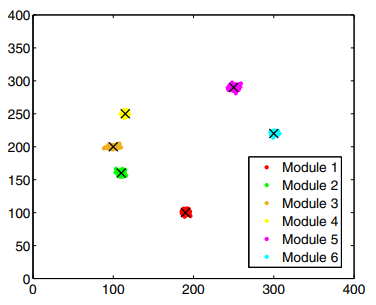
\includegraphics[scale=0.8]{images/impossible.png}
\caption{Plots des clusters pour les 6 modules de l'article\cite{loraDCTF}}\label{term4000}
\end{figure}

 
\section{Méthode DCTF en pratique}\label{pra}

L'analyse suivante est basée sur la section \ref{DCTF}. Cette section a pour but de présenter la méthode \ac{DCTF} sur le matériel qui a été présenté dans le chapitre précédent. Cette section détaille toutes les étapes de la méthode pour un seul appareil avec un seul set de paramètres. Afin de rendre pertinente la méthode, les résultats (sans les étapes intermédiaires) sont présentés dans la section \ref{result}.

Le signal test pour cette analyse est le signal contenant les paramètres suivants :

\vspace{0.1cm}

\begin{itemize}
\item émetteur : module RN2483, modulation : LoRa, \ac{SF} = 8, \ac{BW} = 125KHz, fréquence = 868MHz, power = 14dBm, \ac{CR} = 4/8.
\item Récepteur : RTL SDR R820T2, fréquence = 866MHz, \ac{SR} = 2MHz, gain = 5dB.
\end{itemize}

\begin{figure}[h]
\centering

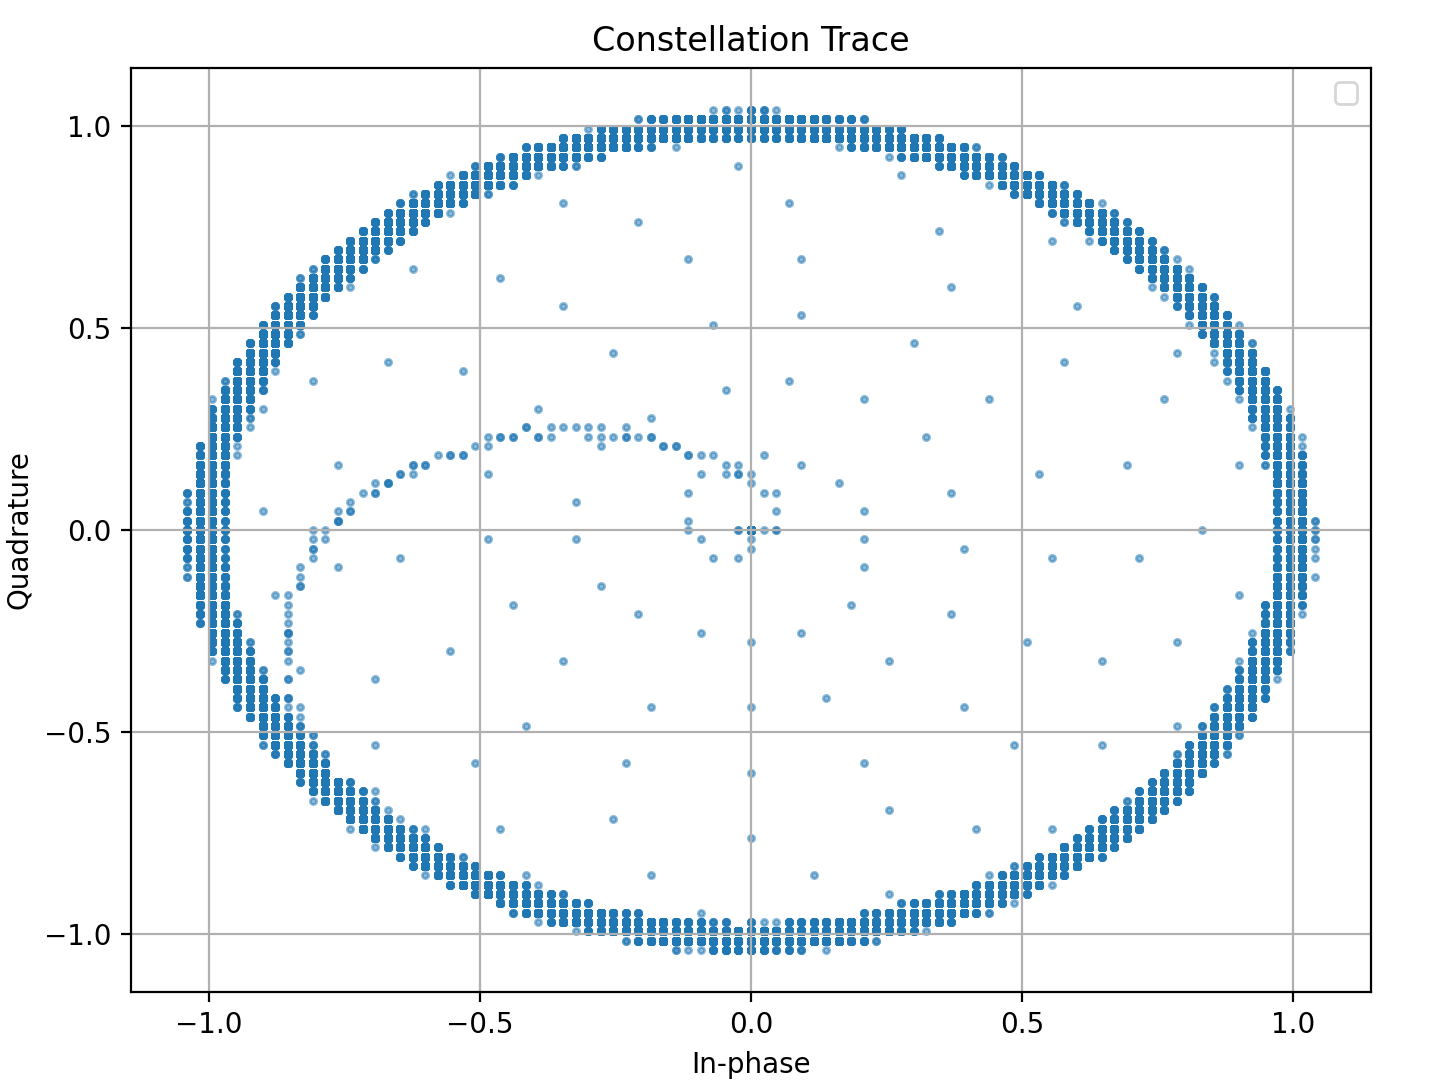
\includegraphics[scale=0.25]{images/dctf1.png}
\caption{Diagramme de constellations}\label{term314}
\end{figure}


La méthode \ac{DCTF} se base sur l'utilisation de constellations traces pour pouvoir identifier sur base de propriétés uniques un appareil. Un diagramme de constellations est une représentation dans le plan complexe de la distribution spaciale des points du signal. La figure \ref{term314} montre la représentation  du signal sous forme de constellations. On remarque que le diagramme forme un cercle contenant la majorité des points. Cependant, certains points dévient vers le centre, ce sont les échantillons correspondant à la partie transitoire (observée à la figure \ref{term307}).

\vspace{0.1cm}

Selon la section \ref{DCTF}, le diagramme de constellations seul n'est pas suffisant pour pouvoir identifier des composantes uniques au signal. Pour pouvoir observer l'émergence d'une signature, il faut appliquer la méthode différentielle décrite par l'équation \ref{eq4003}. La figure \ref{term316} montre le diagramme différentiel de constellations \ac{DCTF} du signal. L'équation \ref{eq1} possède une inconnue, $n$. L'intervalle différentiel se calcule via \ref{eq4006} et vaut 4096 (pour ces paramètres uniquement).


\newpage

\begin{figure}[h]
\centering

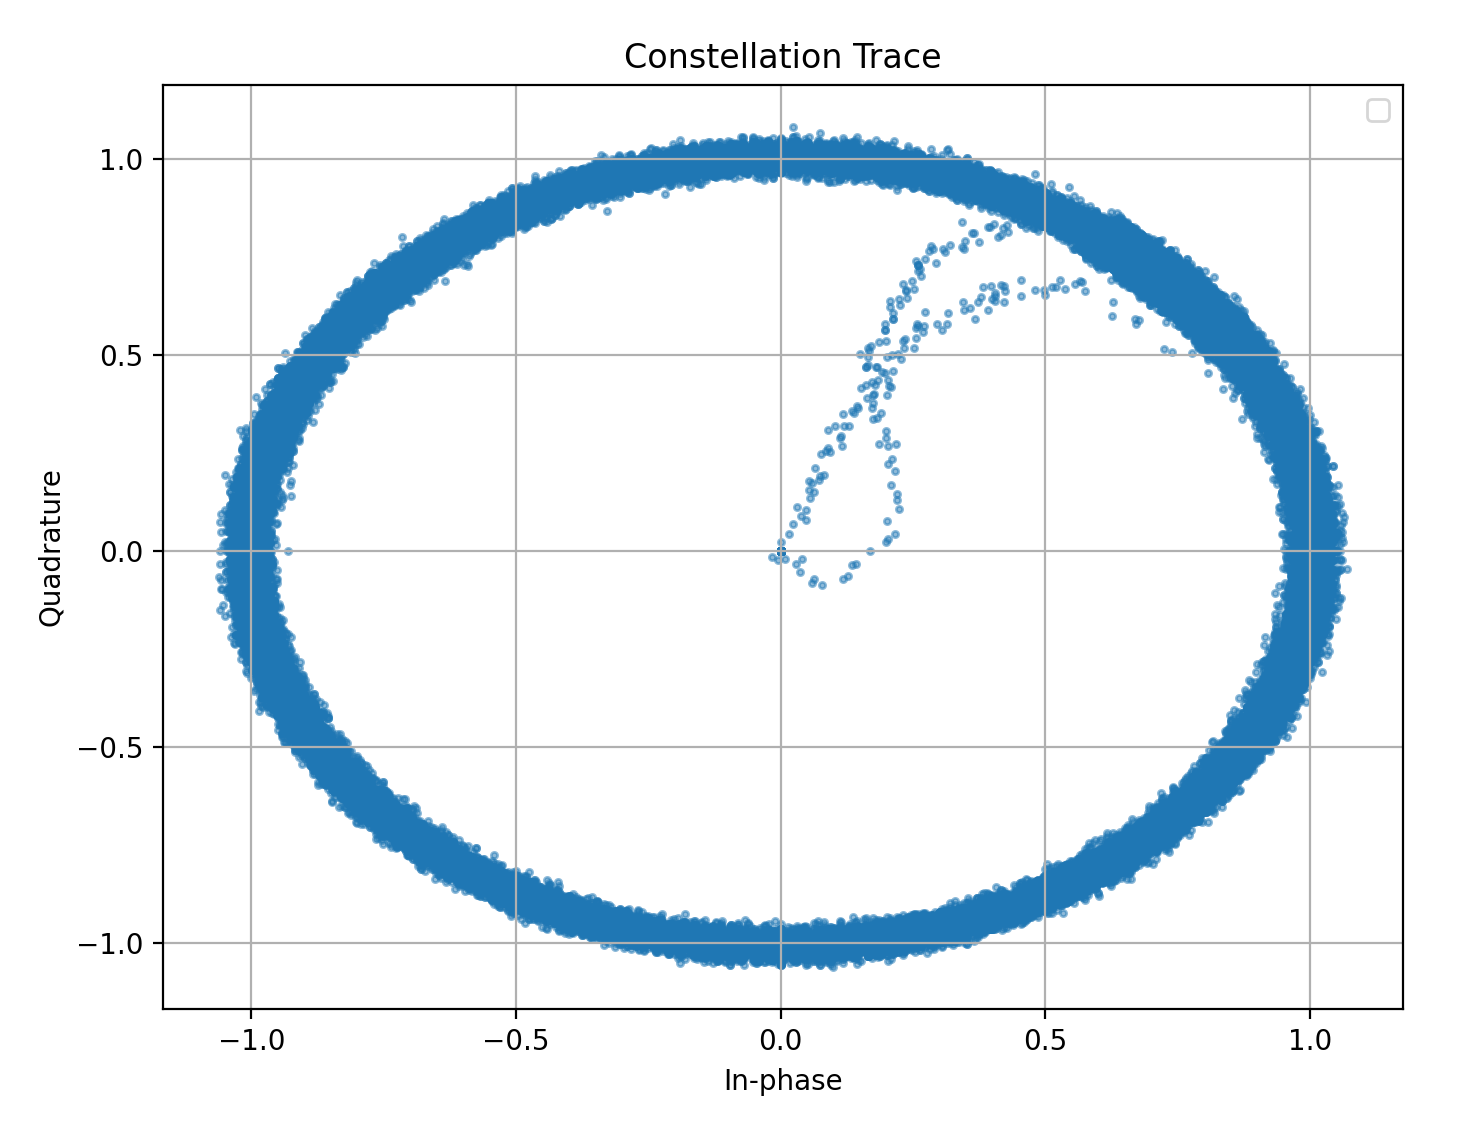
\includegraphics[scale=0.25]{images/dctf3.png}
\caption{DCTF du signal test}\label{term316}
\end{figure}

On remarque que la forme de la constellation est similaire, mais l'application de la méthode différentielle juxtapose les points les uns sur les autres à tel point qu'il devient difficile d'analyser en détails sa composition. Pour pouvoir observer une composante susceptible d'être une signature, il faut appliquer un gradient coloré pour évaluer la densité des points de la constellation. La figure \ref{term317} montre le même diagramme qu'à la figure \ref{term316} mais avec l'utilisation de la librairie Python Datashader, qui ajoute une échelle de densité (en pourcentage, ou 100 représente la zone la plus dense du diagramme). On observe que dans le coin supérieur droit la densité de points est un peu plus élevée que dans le reste de la constellation.

\vspace{0.1cm}

Jusqu'à présent, l'analyse a été faite en utilisant l'intégralité du signal comme donnée. Cependant, l'article \cite{loraDCTF} a montré qu'il est possible de filtrer une partie des données et ainsi ne conserver qu'une partie suffisante du signal pour déterminer sa signature. Premièrement, d'un point de vue physique, le signal possède une partie appelée \textit{transient part}, c'est la portion initiale du signal qui contient la transition d'un état vers un autre.

\newpage

\begin{figure}[h]
\centering

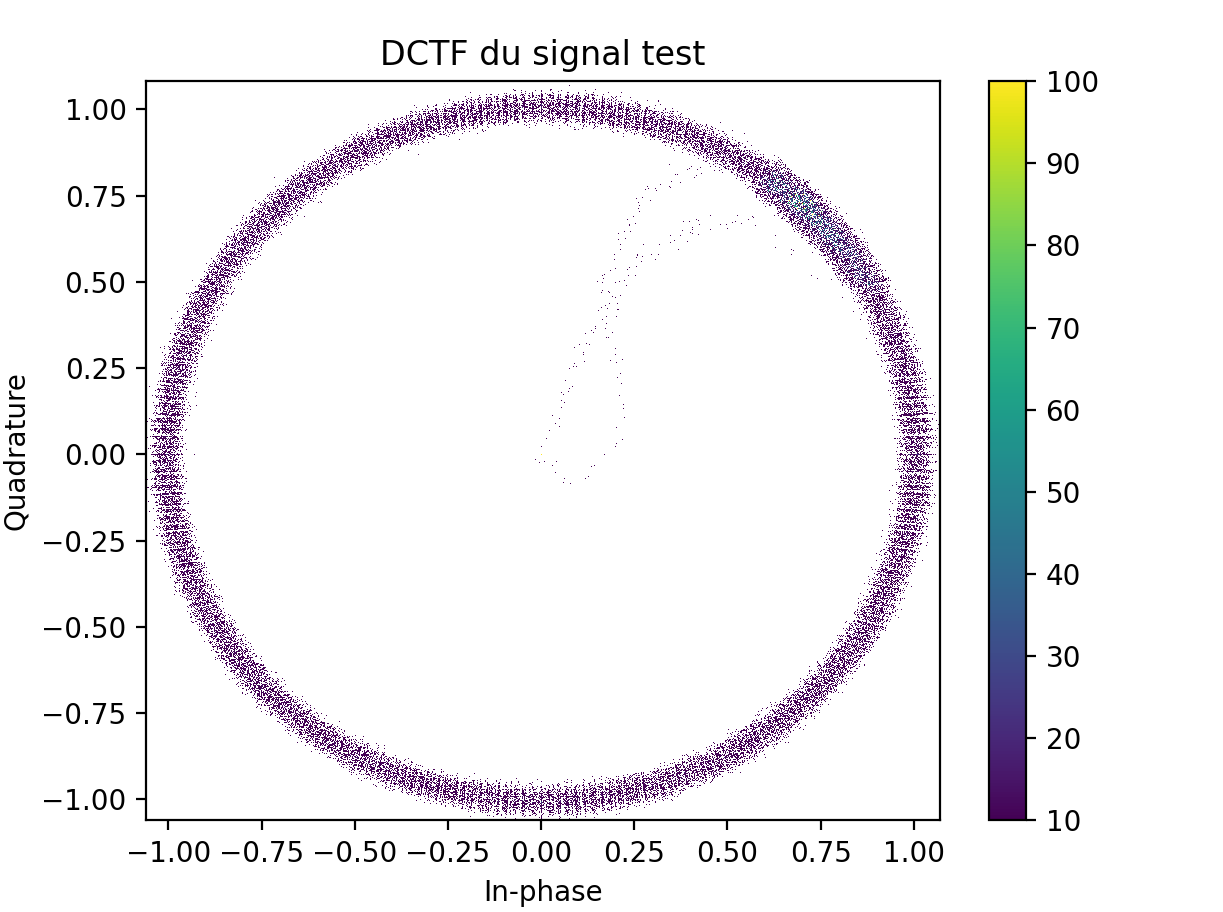
\includegraphics[scale=0.3]{images/dctf4.png}
\caption{DCTF du signal test avec gradient}\label{term317}
\end{figure}

Cette partie se caractérise sur la figure \ref{term317} par les points qui ne se situent pas sur la constellation mais entre la constellation et le centre du plot. La partie transitoire a déja été discutée dans la section \ref{urh}. Cette partie seule étant instable, elle est écartée des données analysées en supprimant de l'analyse une partie du premier chirp du signal. Ensuite, l'intégralité du signal n'est pas nécessaire. En effet, le contenu du message (dans la partie payload du paquet \ac{LoRa}) est sujet à variations et n'est pas pertinent pour l'analyse, seule la partie incluant le préambule est conservée. Ainsi, du signal complet on ne conserve que le préambule (12.25 chirps) auquel on supprime la \textit{transient part} au début des données. La figure \ref{term318} permet de distinguer clairement la région de plus haute densité dans le coin supérieur droit après avoir supprimé les données jugées non pertinentes.

\vspace{0.1cm}

Maintenant que la région d'intérêt est identifiée, il faut l'extraire. C'est ce qui sera extrait de cette \ac{DCTF} qui sera la signature du signal, et donc permettra l'identification du module. Pour déterminer la meilleure valeur dans le plan à récupérer, la méthode suivante permet de récupérer le centre de la zone dense. La librairie Numpy de Python permet de créer un histogramme en deux dimensions de la \ac{DCTF}. Afin d'extraire la valeur la plus pertinente (le centre de la zone dense), le point le plus dense de l'histogramme sert de référentiel. Sa valeur de densité est calculée, c'est à dire le nombre d'échantillons présents dans cette zone définie par l'histogramme. Afin de mieux refléter le centre de la zone dense, tous les points ayant une valeur de densité au moins égale à 90 pour cent (valeur choisie dans l'article \cite{loraDCTF}) de la zone la plus dense sont également considérés. La figure \ref{term319} montre les points sélectionnés pour le signal test dans la \ac{DCTF}. Les coordonnées du centre sont calculées à partir des points éligibles. Ces coordonnées sont celles de la signature du signal. 

\begin{figure}[h]
\centering

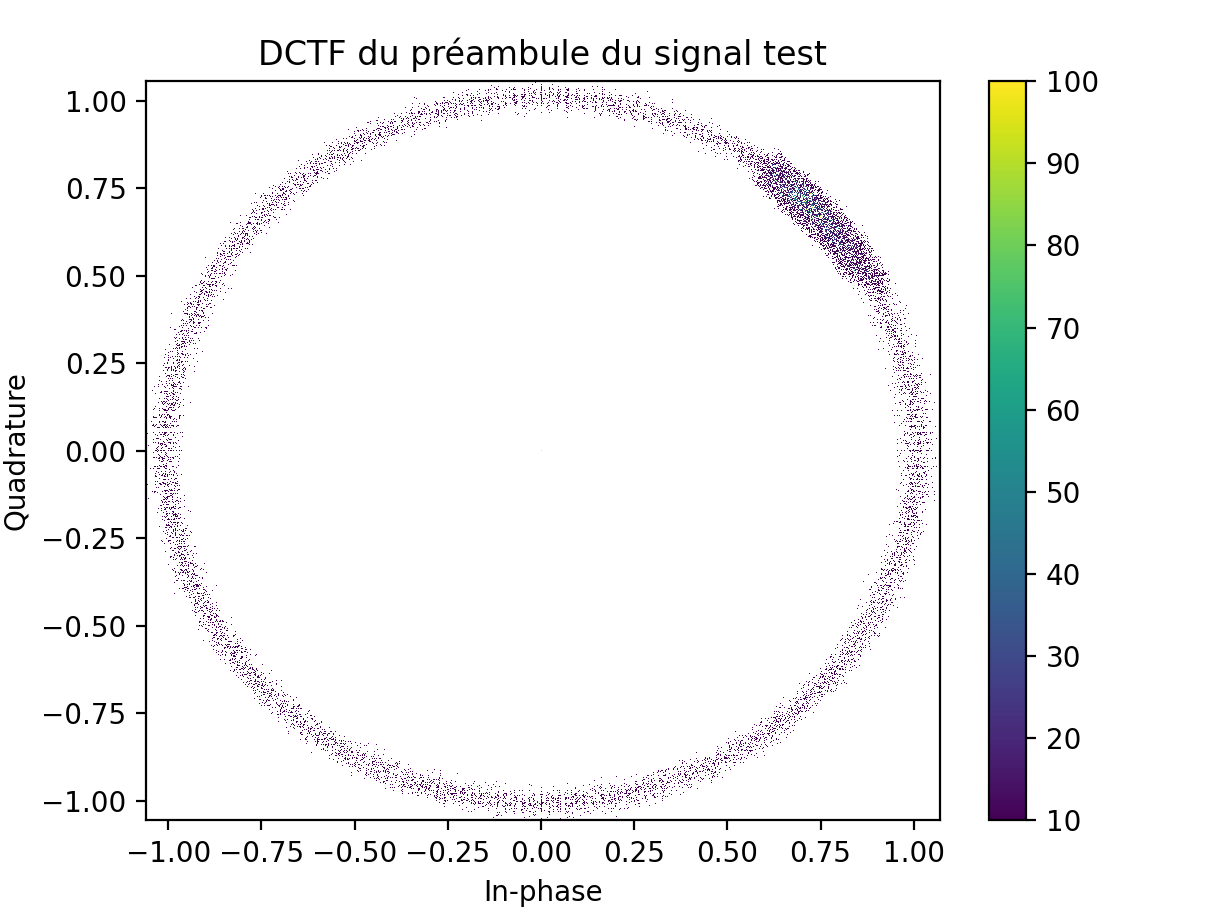
\includegraphics[scale=0.3]{images/dctf5.png}
\caption{DCTF du préambule du signal test avec gradient}\label{term318}
\end{figure}

Finalement, pour obtenir un cluster permettant l'identification de chaque signal provenant ou non du module d'émission, il faut répéter cette opération pour chaque nouveau signal. Selon l'article, la position géographique des centres est relativement proche, ce qui permet de former le cluster de points. Ainsi, en conservant les mêmes paramètres d'émission, 24 autres signaux sont générés avec le même émetteur et la figure \ref{term320} montre les points de chaque signal dans le plan cartésien.

\newpage

\begin{figure}[h]
\centering

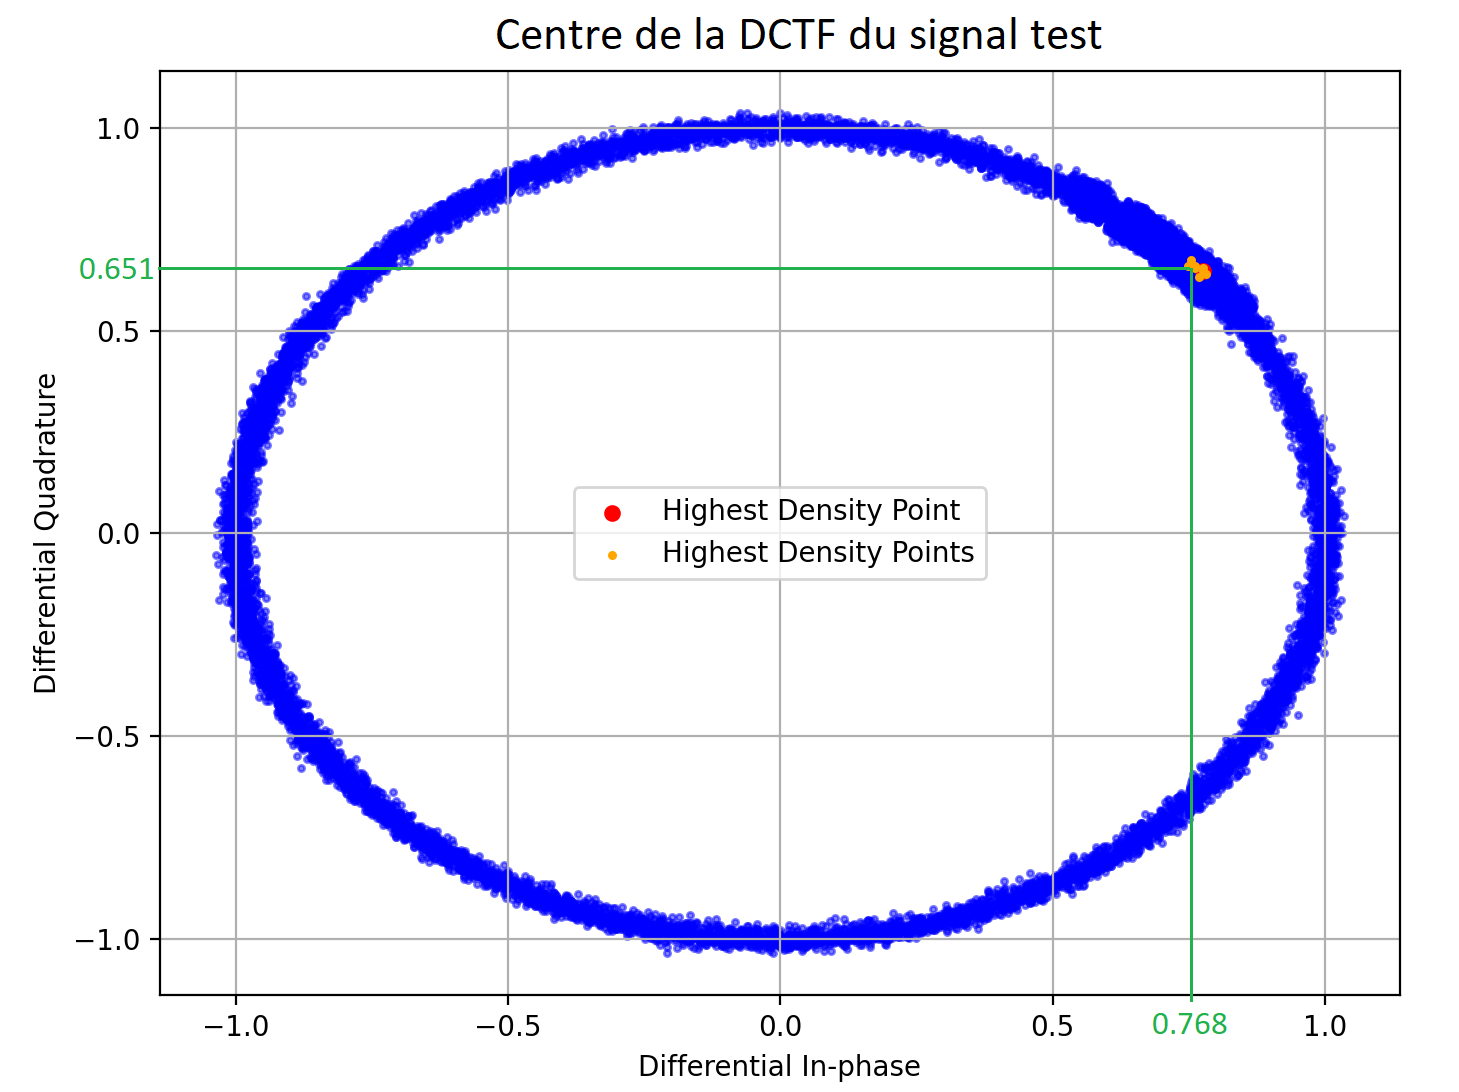
\includegraphics[scale=0.3]{images/dctf6.png}
\caption{Points de haute densité dans la DCTF du signal test}\label{term319}
\end{figure}

\begin{figure}[h]
\centering

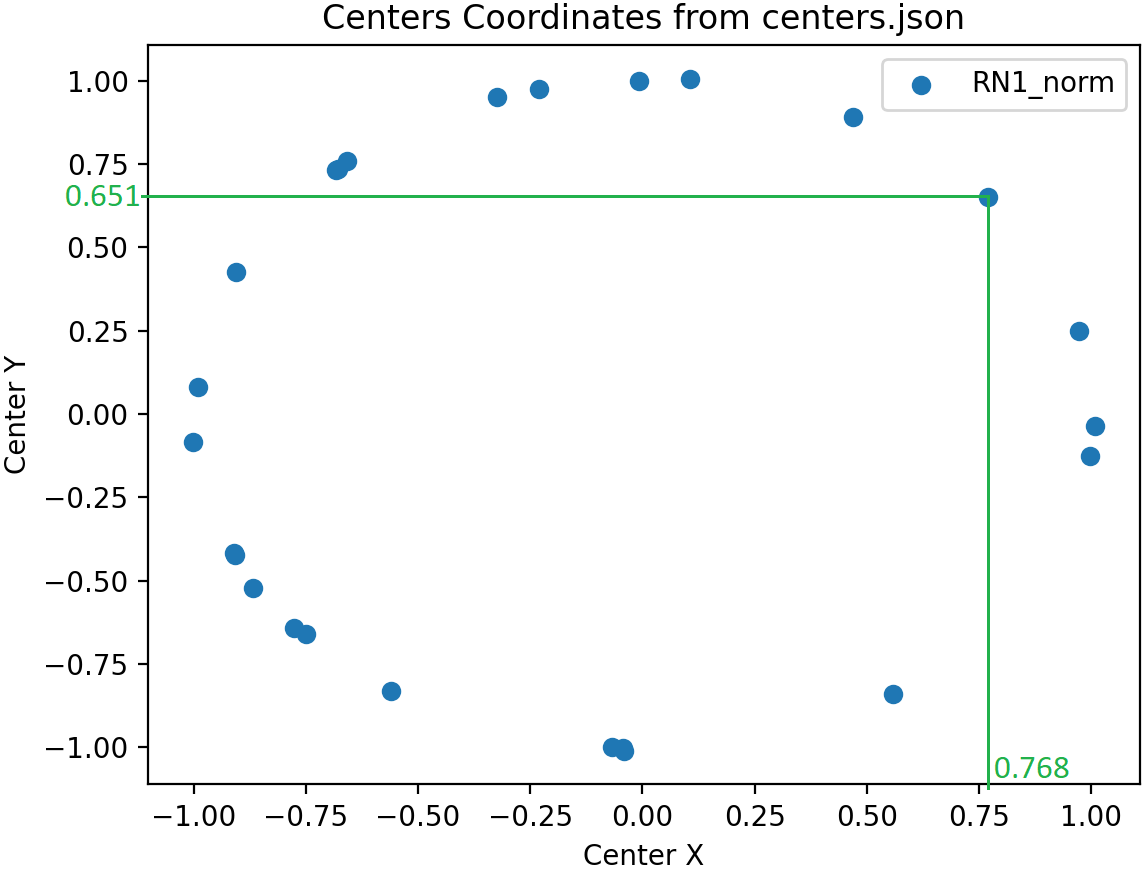
\includegraphics[scale=0.35]{images/cluster.png}
\caption{Répartition des centres des signaux normalisés}\label{term320}
\end{figure}


On remarque que contrairement à l'article et à la figure \ref{term4000}, les points ne forment pas un cluster mais sont en revanche dispersés tout le long du cercle. Afin de déterminer les causes de cette différence de résultats, la section \ref{result} va présenter des alternatives et également tester la méthode sur plusieurs appareils.

\newpage

\section{Résultats}\label{result}

Les résultats obtenus lors de la démonstration à la section  \ref{pra} ne coïncident pas avec ceux de la figure \ref{term4000} de la section \ref{DCTF}. Cette section va, dans un premier temps, proposer différents paramètrages et appareils afin de confirmer les résultats, ou constater des variations en fonction de différents critères. Ensuite, une alternative à l'article sera évoquée mais encore basée sur la signature mise en évidence dans la section \ref{DCTF}. 

Ainsi, 3 appareils sont désormais choisis pour réappliquer la méthode \ref{DCTF}. Afin d'approfondir l'analyse, plusieurs paramétrages différents ont été testés sur chacun des émetteurs. La table \ref{set} donne tous les sets de paramètres qui ont été testés. Les variations impliquent le facteur d'étalement, la largeur de bande du signal ainsi que le taux d'échantillonage. Afin de tenter d'analyser le comportement de la \ac{DCTF}, des dégradations sur le signal sont aussi ajoutées. Une dégradation est basée sur la saturation du signal par un gain trop élevé à la réception par la \ac{SDR}. Une autre dégradation est basée sur une perte importante d'une partie des données. Une dernière est basée sur des variations de l'amplitude du signal, en réduisant successivement l'amplitude durant chaque chirp.

\begin{table}[h]
\centering
\begin{tabular}{|c|c|c|c|p{3cm}|c|}
\hline
Set \# & BW & SF & SR & Qualité du signal & Nombre d'échantillons\\
\hline
1  & 125kHz & 7 & 2 MHz & Elevée & 25\\
\hline
2  & 125kHz & 8 & 2 MHz & Elevée & 25\\
\hline
3  & 125kHz & 9 & 2 MHz & Elevée & 25\\
\hline
4  & 125kHz & 10 & 2 MHz & Elevée & 25\\
\hline
5  & 125kHz & 11 & 2 MHz & Elevée & 25\\
\hline
6  & 125kHz & 12 & 2 MHz & Elevée & 25\\
\hline
7  & 250kHz & 8 & 2 MHz & Elevée & 25\\
\hline
8  & 250kHz & 8 & 1 MHz & Elevée & 25\\
\hline
9  &  125kHz & 8 & 2 MHz & faible (saturation par gain) & 25\\
\hline
10  & 125kHz & 8 & 2 MHz & faible (perte de 50\% du signal) & 5\\
\hline
11  & 125kHz & 8 & 2 MHz & faible (variation de l'amplitude) & 5\\
\hline
\end{tabular}
\caption{Table des paramètres}
\label{set}
\end{table}

Les tables \ref{signature1}, \ref{signature2} et \ref{signature3} montrent pour chaque set de la table \ref{set} s'il est possible d'obtenir un cluster de points pour chaque module. Les tables fournissent des informations concernant la position et la forme de la signature si cette dernière est identifiable.

\newpage

\begin{table}[h]
\centering
\begin{tabular}{|c|c|c|c|c|}
\hline
Set \# & signature identifiable & position & forme & cluster possible\\
\hline
1 & oui & variable & 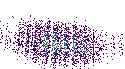
\includegraphics[scale=0.2]{images/set1.png} & non \\
\hline
2 & oui & variable & 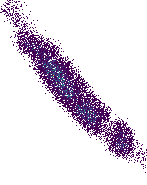
\includegraphics[scale=0.2]{images/set2.png} & non \\
\hline
3 & oui & variable & 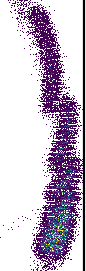
\includegraphics[scale=0.35]{images/set3.png} & non \\
\hline
4 & oui & variable & 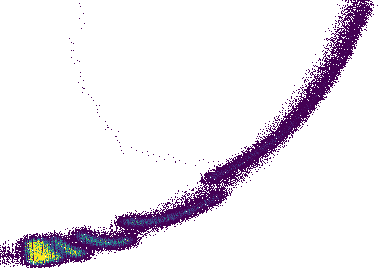
\includegraphics[scale=0.2]{images/set4.png} & non \\
\hline
5 & oui & variable & 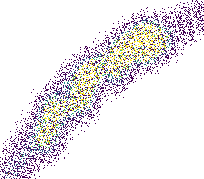
\includegraphics[scale=0.2]{images/set5.png} & non \\
\hline
6 & oui & variable & 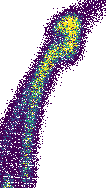
\includegraphics[scale=0.2]{images/set6.png} & non \\
\hline
7 & oui & variable & 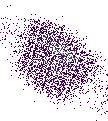
\includegraphics[scale=0.2]{images/set7.png} & non \\
\hline
8 & oui & variable & 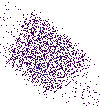
\includegraphics[scale=0.2]{images/set8.png} & non \\
\hline
9 & oui & variable & variable & non \\
\hline
10 & non & inconnu & inconnu  & non \\
\hline
11 & oui & variable & 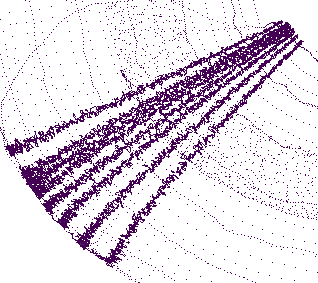
\includegraphics[scale=0.2]{images/set11.png}  & non \\
\hline
\end{tabular}
\caption{Table des caractéristiques de la signature pour le device RN2483 \#1}
\label{signature1}
\end{table}

On remarque, dans la table \ref{signature1}, qu'augmenter le spreading factor altère fortement la forme de la signature. Elle s'apparente à une comète tournant le long de la \ac{DCTF} dont la queue s'étend avec le spreading factor. Sa position est variable dans le diagramme, mais sa forme est similaire pour un SF fixé. Modifier la lageur de bande n'a pas d'impact sur la signature (sa position ou sa forme). Réduire le taux d'échantillonage réduit la netteté de la constellation, donc le taux d'échantillonnage affecte la densité de la \ac{DCTF} sans modifier sa forme ou sa position. La détérioration du signal a des conséquences variables sur la \ac{DCTF}. Saturer le signal provoque une dégradation importante du cercle, à tel point que la forme de la signature devient également variable. Une perte trop importante du signal entraine tout simplement la disparation de la signature. Finalement, les variations d'amplitude font converger les points vers le centre de la \ac{DCTF}, ce qui donne une projection de la signature étirée vers le centre. Cette anomalie, citée à la section \ref{DCTF} est bien confirmée dans les expérimentations.

\begin{table}[h]
\centering
\begin{tabular}{|c|c|c|c|c|}
\hline
Set \# & signature & position & forme & cluster\\
 & identifiable & & & possible\\
\hline
1 & oui & variable & 
\includegraphics[scale=0.2]{images/set12.png}  & non \\
\hline
2 & oui & variable & 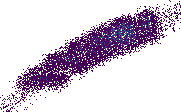
\includegraphics[scale=0.2]{images/set13.png}  & non \\
\hline
3 & oui & variable & 
\includegraphics[scale=0.35]{images/set14.png}  & non \\
\hline
4 & oui & variable & 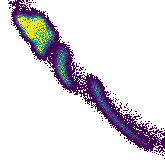
\includegraphics[scale=0.2]{images/set15.png}  & non \\
\hline
5 & oui & variable & 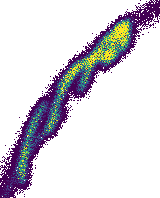
\includegraphics[scale=0.2]{images/set16.png}  & non \\
\hline
6 & non & multiples & 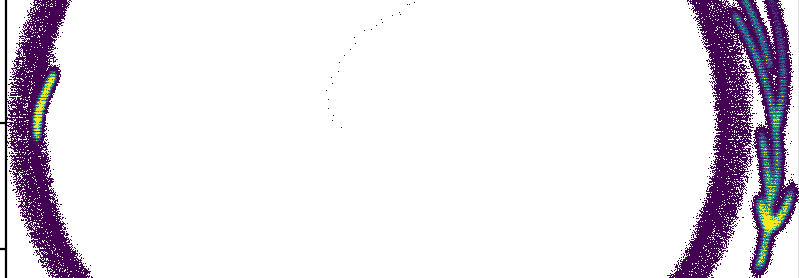
\includegraphics[scale=0.35]{images/set17.png}  & non \\
\hline
7 & oui & variable & 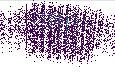
\includegraphics[scale=0.2]{images/set18.png}  & non \\
\hline
8 & oui & variable & 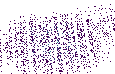
\includegraphics[scale=0.2]{images/set19.png}  & non \\
\hline
9 & non & inconnu & inconnu & non \\
\hline
10 & non & inconnu & inconnu  & non \\
\hline
11 & non & variable & 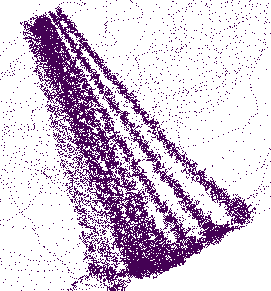
\includegraphics[scale=0.2]{images/set22.png}  & non \\
\hline
\end{tabular}
\caption{Table des caractéristiques de la signature pour le device RN2483 \#2}
\label{signature2}
\end{table}

La plupart des commentaires sur la première table sont valables pour la table \ref{signature2}. Cependant, on constate qu'un spreading factor maximal (\ac{SF} = 12) génère une seconde signature. On remarque également que la signature se trouve à l'extérieur du cercle.

\newpage

\begin{table}[h]
\centering
\begin{tabular}{|c|c|c|c|c|}
\hline
Set \# & signature identifiable & position & forme & cluster possible\\
\hline
1 & oui & variable & 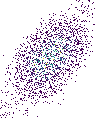
\includegraphics[scale=0.2]{images/set23.png}  & non \\
\hline
2 & oui & variable & 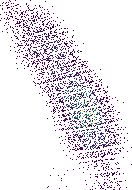
\includegraphics[scale=0.2]{images/set24.png}  & non \\
\hline
3 & oui & variable & 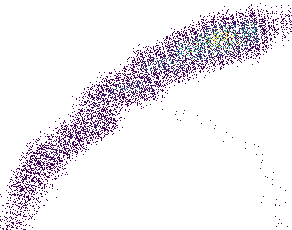
\includegraphics[scale=0.2]{images/set25.png}  & non \\
\hline
4 & oui & variable & 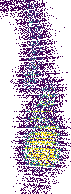
\includegraphics[scale=0.2]{images/set26.png}  & non \\
\hline
5 & oui & multiples & 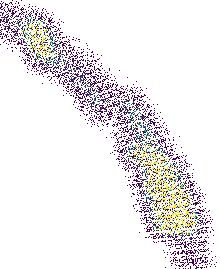
\includegraphics[scale=0.2]{images/set27.png}  & non \\
\hline
6 & oui & variable & 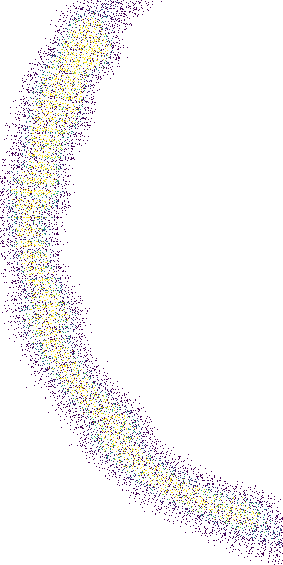
\includegraphics[scale=0.1]{images/set28.png}  & non \\
\hline
7 & non & inconnu & inconnu & non \\
\hline
8 & non & inconnu & inconnu & non \\
\hline
9 & non & inconnu & inconnu & non \\
\hline
10 & non & inconnu & inconnu  & non \\
\hline
11 & non & multiples & 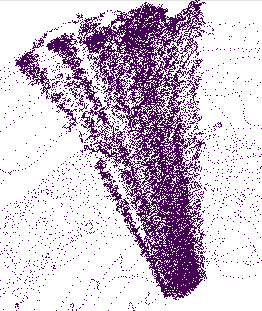
\includegraphics[scale=0.2]{images/set33.png}  & non \\
\hline
\end{tabular}
\caption{Table des caractéristiques de la signature pour le device RN2483 \#3}
\label{signature3}
\end{table}

La dernière table \ref{signature3} confirme les éléments analysés dans les tables \ref{signature1} et \ref{signature2}. Les signaux de ce module sont cependant moins nets, ce qui entraine des signatures moins denses, plus difficiles à repérer, voire carrément absentes.

\vspace{0.1cm}

Selon les résultats des tables \ref{signature1}, \ref{signature2} et \ref{signature3}, il n'est pas possible de pouvoir identifier un noeud émetteur \ac{LoRa} en se basant sur la position de la signature dans la \ac{DCTF} du signal analysé. Cependant, une autre possibilté non mentionnée par l'article s'est révélée durant les expérimentations. Si la position de la signature pour un même set de paramètres est variable, sa forme en revanche, est similaire. 

Mieux encore, pour deux noeuds différents ayant les mêmes paramètres, on peut constater des différences dans la forme des signatures. \textbf{Il existe donc bel et bien une propriété physique unique associée à chaque signal qui permettrait d'identifier son noeud émetteur}. La table \ref{compa} montre les signatures capturées de 6 échantillons différents pour chacun des modules testés. Le set choisi pour la comparaison est le set \#4

\begin{table}[h]
\centering
\begin{tabular}{|c|c|c|c|}
\hline
échantillons \# & module \#1 & module \#2 & module \#3\\
\hline
1 & 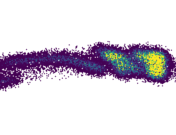
\includegraphics[scale=0.4]{images/m11.png} & 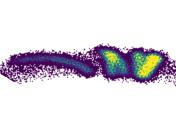
\includegraphics[scale=0.4]{images/m21.png} & 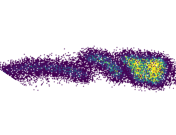
\includegraphics[scale=0.4]{images/m31.png}  \\
\hline
2 & 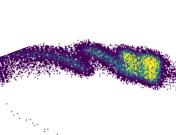
\includegraphics[scale=0.4]{images/m12.png} & 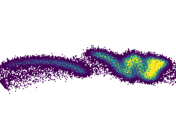
\includegraphics[scale=0.4]{images/m22.png} & 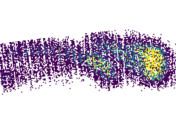
\includegraphics[scale=0.4]{images/m32.png}  \\
\hline
3 & 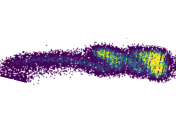
\includegraphics[scale=0.4]{images/m13.png} & 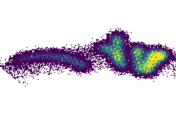
\includegraphics[scale=0.4]{images/m23.png} & 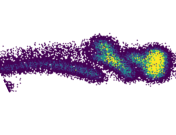
\includegraphics[scale=0.4]{images/m33.png} \\
\hline
4 & 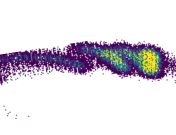
\includegraphics[scale=0.4]{images/m14.png} & 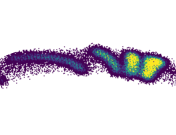
\includegraphics[scale=0.4]{images/m24.png} & 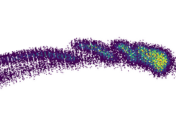
\includegraphics[scale=0.4]{images/m34.png}  \\
\hline
5 & 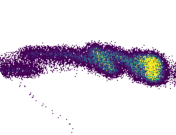
\includegraphics[scale=0.4]{images/m15.png} & 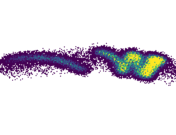
\includegraphics[scale=0.4]{images/m25.png} & 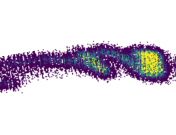
\includegraphics[scale=0.4]{images/m35.png}  \\
\hline
6 & 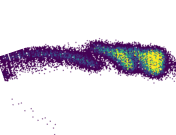
\includegraphics[scale=0.4]{images/m16.png} & 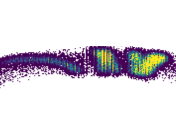
\includegraphics[scale=0.4]{images/m26.png} & 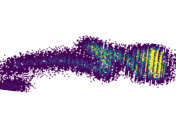
\includegraphics[scale=0.4]{images/m36.png}  \\
\hline
\hline
forme générale & \includegraphics[scale=0.2]{images/gen1.png} & \includegraphics[scale=0.2]{images/gen2.png} & \includegraphics[scale=0.2]{images/gen3.png} \\
\hline
\end{tabular}
\caption{Table comparative des formes géométriques des signatures pour le set \#4}
\label{compa}
\end{table}

Même si dans un premier temps les signatures ont des formes proches, s'apparentant à des comètes, il y a cepedant des différences notables entre chaque module. En effet, les signatures du premier module ont une tête de comète arrondie, là où celles du second module ont une finition pointue. La queue de la comète des signatures du second module est systématiquement détachée du reste du corps. La tête de la comète des signatures du troisème module est plus grosse que les deux autres, avec un corps plus étendu.